\documentclass[aspectratio=169]{beamer}
\usetheme{Madrid}
\usecolortheme{default}

\usepackage{graphicx}
\usepackage{listings}
\usepackage{xcolor}
\usepackage{tikz}
\usepackage{enumitem}

\title{Kitchensink User Management Platform}
\subtitle{Enterprise-Grade User Management with Security \& Scalability}
\author{Product Overview}
\date{\today}

\begin{document}

% Slide 1: Title
\frame{\titlepage}

% Slide 2: Overview
\begin{frame}{Overview}
    \begin{itemize}[leftmargin=*]
        \item \textbf{Enterprise User Management System} - Secure, scalable platform for managing millions of users
        \item \textbf{Migrated from Jakarta EE} to modern Spring Boot architecture
        \item \textbf{Full-Stack Solution}: Spring Boot REST API + React Frontend
        \item \textbf{Production-Ready} with comprehensive security, monitoring, and audit capabilities
        \item \textbf{NoSQL Database} (MongoDB) for horizontal scalability
    \end{itemize}
    \vspace{0.5cm}
    \begin{block}{Core Purpose}
        Secure user registration, authentication, profile management, and administrative operations with enterprise-grade security and compliance features.
    \end{block}
\end{frame}

% Slide 3: Key Features
\begin{frame}{Key Features}
    \begin{columns}
        \column{0.5\textwidth}
        \textbf{User Management}
        \begin{itemize}
            \item User registration \& authentication
            \item OTP-based login system
            \item Profile management (self \& admin)
            \item Role-based access control (RBAC)
            \item Cursor-based pagination
            \item Advanced search \& filtering
        \end{itemize}
        
        \column{0.5\textwidth}
        \textbf{Administrative Features}
        \begin{itemize}
            \item Admin dashboard
            \item Update request workflow
            \item User approval/rejection
            \item Audit trail \& logging
            \item Email notifications
            \item Correlation ID tracking
        \end{itemize}
    \end{columns}
\end{frame}

% Slide 4: Technology Stack
\begin{frame}{Technology Stack}
    \begin{columns}
        \column{0.5\textwidth}
        \textbf{Backend}
        \begin{itemize}
            \item Java 21, Spring Boot 3.5.7
            \item Spring Data MongoDB
            \item Spring Security + JWT
            \item Caffeine Cache
            \item Jasypt (PII Encryption)
            \item Spring Actuator (Monitoring)
        \end{itemize}
        
        \column{0.5\textwidth}
        \textbf{Frontend \& Database}
        \begin{itemize}
            \item React 18
            \item MongoDB 8.0+ (NoSQL)
            \item Axios for API calls
            \item Modern responsive UI
        \end{itemize}
        
        \vspace{0.3cm}
        \textbf{DevOps \& Tools}
        \begin{itemize}
            \item Maven (Build)
            \item Swagger/OpenAPI
            \item Prometheus metrics
            \item Logback logging
        \end{itemize}
    \end{columns}
\end{frame}

% Slide 5: Security Features
\begin{frame}{Security Features}
    \begin{enumerate}[leftmargin=*]
        \item \textbf{Authentication \& Authorization}
        \begin{itemize}
            \item JWT-based stateless authentication
            \item OTP verification for login
            \item Role-based access control (ADMIN/USER)
            \item API key authentication (optional)
        \end{itemize}
        
        \item \textbf{Data Protection}
        \begin{itemize}
            \item PII encryption (email, phone) using Jasypt
            \item Encrypted storage in MongoDB
            \item Decryption only at service layer
            \item Legacy key support for key rotation
        \end{itemize}
        
        \item \textbf{Input Security}
        \begin{itemize}
            \item Input sanitization (XSS prevention)
            \item SQL injection protection (NoSQL safe)
            \item Request validation
        \end{itemize}
    \end{enumerate}
\end{frame}

% Slide 6: Security Limits \& Configuration
\begin{frame}{Security Limits \& Configuration}
    \begin{block}{Rate Limiting}
        \begin{itemize}
            \item \textbf{API Requests}: 60/minute, 1000/hour per IP
            \item \textbf{OTP Generation}: 1000 attempts per 15-minute window
            \item \textbf{OTP Verification}: Max 5 failed attempts, 15-minute lockout
            \item Failed attempts stored in MongoDB with auto-cleanup
        \end{itemize}
    \end{block}
    
    \begin{block}{Session \& Token Security}
        \begin{itemize}
            \item JWT expiration: 24 hours (86400000 ms)
            \item Stateless sessions (no server-side storage)
            \item CORS protection with whitelisted origins
        \end{itemize}
    \end{block}
    
    \begin{block}{Cache Security}
        \begin{itemize}
            \item Only encrypted PII stored in cache (UserCacheDTO)
            \item Cache eviction on updates/deletes
            \item TTL-based expiration (3-15 minutes)
        \end{itemize}
    \end{block}
\end{frame}

% Slide 7: Architecture Overview
\begin{frame}{Architecture Overview}
    \begin{center}
        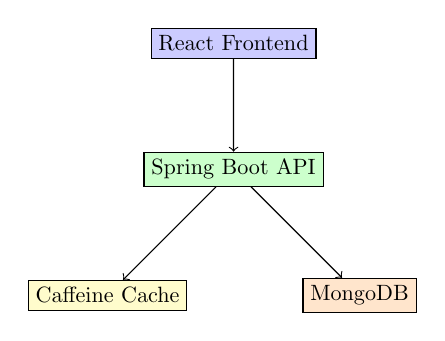
\begin{tikzpicture}[scale=0.8, transform shape]
            \node[draw, rectangle, fill=blue!20] (client) at (0,4) {React Frontend};
            \node[draw, rectangle, fill=green!20] (api) at (0,2) {Spring Boot API};
            \node[draw, rectangle, fill=yellow!20] (cache) at (-2,0) {Caffeine Cache};
            \node[draw, rectangle, fill=orange!20] (db) at (2,0) {MongoDB};
            
            \draw[->] (client) -- (api);
            \draw[->] (api) -- (cache);
            \draw[->] (api) -- (db);
        \end{tikzpicture}
    \end{center}
    
    \vspace{0.3cm}
    \textbf{Request Flow:}
    \begin{enumerate}
        \item Correlation ID Filter $\rightarrow$ Rate Limiting $\rightarrow$ Authentication
        \item Controller $\rightarrow$ Service Layer $\rightarrow$ Cache Check
        \item Repository $\rightarrow$ MongoDB Query $\rightarrow$ Response
    \end{enumerate}
\end{frame}

% Slide 8: Data Management
\begin{frame}{Data Management}
    \begin{columns}
        \column{0.5\textwidth}
        \textbf{PII Encryption}
        \begin{itemize}
            \item Email \& phone encrypted at rest
            \item AES encryption with configurable keys
            \item Key versioning for rotation
            \item Decryption only when needed
        \end{itemize}
        
        \textbf{Caching Strategy}
        \begin{itemize}
            \item Caffeine in-memory cache
            \item User cache: 500 entries, 3min TTL
            \item Role cache: 50 entries, 15min TTL
            \item Cache-aside pattern
        \end{itemize}
        
        \column{0.5\textwidth}
        \textbf{MongoDB Collections}
        \begin{itemize}
            \item \texttt{users} - User profiles
            \item \texttt{roles} - Role definitions
            \item \texttt{user\_roles} - Role assignments
            \item \texttt{otps} - OTP storage
            \item \texttt{update\_requests} - Change requests
            \item \texttt{audit\_logs} - Audit trail
            \item \texttt{otp\_verification\_attempts} - Rate limiting
        \end{itemize}
    \end{columns}
\end{frame}

% Slide 9: Authentication \& Authorization
\begin{frame}{Authentication \& Authorization}
    \textbf{OTP-Based Login Flow:}
    \begin{enumerate}
        \item User requests OTP via email
        \item System generates 6-digit OTP (15min expiry)
        \item OTP sent via email service
        \item User submits OTP for verification
        \item On success: JWT token issued
        \item Rate limiting prevents brute force
    \end{enumerate}
    
    \vspace{0.3cm}
    \textbf{Role-Based Access:}
    \begin{itemize}
        \item \textbf{ADMIN}: Full access to user management, update requests
        \item \textbf{USER}: Self-profile management only
        \item Method-level security with \texttt{@PreAuthorize}
        \item URL-based access control
    \end{itemize}
\end{frame}

% Slide 10: Audit \& Monitoring
\begin{frame}{Audit \& Monitoring}
    \begin{columns}
        \column{0.5\textwidth}
        \textbf{Audit Logging}
        \begin{itemize}
            \item All user CRUD operations logged
            \item Field-level change tracking
            \item Correlation ID for request tracing
            \item IP address \& timestamp tracking
            \item Async logging (non-blocking)
        \end{itemize}
        
        \column{0.5\textwidth}
        \textbf{Monitoring \& Health}
        \begin{itemize}
            \item Spring Actuator endpoints
            \item Prometheus metrics export
            \item Health checks (DB, cache)
            \item Request/response logging
            \item Performance metrics
        \end{itemize}
    \end{columns}
    
    \vspace{0.3cm}
    \begin{block}{Update Request Workflow}
        Users request profile changes $\rightarrow$ Admin reviews $\rightarrow$ Approve/Reject $\rightarrow$ Email notification $\rightarrow$ Audit log
    \end{block}
\end{frame}

% Slide 11: Scaling to 100M Users - Strategy
\begin{frame}{Scaling to 100M Users - Strategy}
    \textbf{Phase 1: Horizontal Scaling (0-10M users)}
    \begin{itemize}
        \item \textbf{Application Tier}: Multiple Spring Boot instances behind load balancer
        \item \textbf{Database}: MongoDB replica set (1 primary, 2+ secondaries)
        \item \textbf{Cache}: Distributed cache (Redis Cluster)
        \item \textbf{Session}: Stateless JWT (no session store needed)
    \end{itemize}
    
    \textbf{Phase 2: Sharding (10M-100M users)}
    \begin{itemize}
        \item \textbf{MongoDB Sharding}: Shard by user ID or geographic region
        \item \textbf{Read Replicas}: Separate read/write operations
        \item \textbf{Cache Partitioning}: Consistent hashing for Redis
        \item \textbf{CDN}: Static assets and API responses
    \end{itemize}
\end{frame}

% Slide 12: Scaling - Infrastructure
\begin{frame}{Scaling - Infrastructure \& Database}
    \begin{columns}
        \column{0.5\textwidth}
        \textbf{Application Layer}
        \begin{itemize}
            \item \textbf{Kubernetes} orchestration
            \item Auto-scaling (CPU/memory based)
            \item Health checks \& rolling updates
            \item API Gateway (Kong/AWS API Gateway)
        \end{itemize}
        
        \textbf{Database Optimizations}
        \begin{itemize}
            \item \textbf{MongoDB Atlas} or self-hosted cluster
            \item Sharded cluster (10-20 shards)
            \item Sharding key: User ID hash
            \item TTL indexes for auto-cleanup
        \end{itemize}
        
        \column{0.5\textwidth}
        \textbf{Caching Strategy}
        \begin{itemize}
            \item \textbf{Redis Cluster}: Distributed cache
            \item Cache partitioning by user ID
            \item Multi-level cache (L1 + L2)
            \item Event-driven cache eviction
        \end{itemize}
        
        \textbf{Estimated Infrastructure}
        \begin{itemize}
            \item \textbf{App Servers}: 20-50 instances
            \item \textbf{Database}: 10-20 shards, 3 replicas each
            \item \textbf{Cache}: Redis Cluster (6-12 nodes)
            \item \textbf{Load Balancer}: AWS ALB/NGINX
        \end{itemize}
    \end{columns}
\end{frame}

% Slide 13: Additional Scaling Considerations
\begin{frame}{Additional Scaling Considerations}
    \begin{columns}
        \column{0.5\textwidth}
        \textbf{Performance Optimizations}
        \begin{itemize}
            \item Async processing (email, audit)
            \item Database connection pooling
            \item Cursor-based pagination
            \item Batch operations for admin
        \end{itemize}
        
        \textbf{Monitoring \& Observability}
        \begin{itemize}
            \item APM (New Relic, Datadog)
            \item Centralized logging (ELK)
            \item Prometheus + Grafana
            \item Alerting (PagerDuty)
        \end{itemize}
        
        \column{0.5\textwidth}
        \textbf{Security at Scale}
        \begin{itemize}
            \item WAF (AWS WAF, Cloudflare)
            \item DDoS protection
            \item Distributed rate limiting (Redis)
            \item Key rotation automation
        \end{itemize}
        
        \vspace{0.3cm}
        \begin{block}{Current Capacity}
            \begin{itemize}
                \item Single instance: $\sim$10K-50K users
                \item Rate limit: 60 req/min, 1000 req/hour
                \item Cache: 500 users, 50 roles
            \end{itemize}
        \end{block}
    \end{columns}
\end{frame}

% Slide 14: Summary
\begin{frame}{Summary}
    \begin{block}{Key Strengths}
        \begin{itemize}
            \item Enterprise-grade security (encryption, RBAC, rate limiting)
            \item Scalable architecture (stateless, NoSQL, caching)
            \item Comprehensive audit \& monitoring
            \item Production-ready with modern tech stack
        \end{itemize}
    \end{block}
    
    \begin{block}{Scaling Path to 100M Users}
        \begin{enumerate}
            \item Horizontal scaling (load balancer, multiple instances)
            \item Distributed caching (Redis Cluster)
            \item MongoDB sharding \& replica sets
            \item Infrastructure automation (Kubernetes)
            \item Performance monitoring \& optimization
        \end{enumerate}
    \end{block}
    
    \vspace{0.3cm}
    \textbf{Estimated Timeline:} 6-12 months with dedicated DevOps team
\end{frame}

\end{document}

